
\documentclass{article}
\usepackage{graphicx}
\usepackage[pdftex,bookmarks,bookmarksnumbered,colorlinks]{hyperref}
\usepackage{pdfpages}
\usepackage{fancyhdr}
\usepackage[english]{babel}
\usepackage{multicol}
\usepackage[margin=1.1in]{geometry}
\usepackage{textcomp}
\usepackage{fmtcount}
\usepackage[utf8]{inputenc}
\usepackage{hyperref}

%Prevents Tables from being repositioned
\usepackage{float}
\restylefloat{table}

% Table spacing
%Top space
\newcommand{\Toprule}{\rule{0pt}{3.0ex}}
%Bottom space
\newcommand{\Botrule}{\rule[-1.2ex]{0pt}{0pt}}

%Constants
\newcommand{\DocTitle}{ARC FLASH HAZARD ANALYSIS}
\newcommand{\Customer}{Fanshawe College}
\newcommand{\Building}{B Building}
\newcommand{\Address}{123 ur Face}
\newcommand{\JobNum}{2940}


%hyperlinks
\hypersetup{
pdftoolbar=true,        								% show Acrobat�s toolbar?
pdfmenubar=true,        								% show Acrobat�s menu?
pdffitwindow=false,     								% window fit to page when opened
pdfstartview={FitH},    								% fits the width of the page to the window
pdftitle={\DocTitle},    								% title
pdfauthor={PowerCore Engineering},    					% author
pdfsubject={Report},   									% subject of the document
pdfcreator={PowerCore Engineering},   					% creator of the document
pdfproducer={PowerCore Engineering}, 					% producer of the document
pdfnewwindow=true,      								% links in new window
colorlinks=true,       									% false: boxed links; true: colored links
linkcolor=black,          								% color of internal links (change box color with linkbordercolor)
citecolor=blue,        									% color of links to bibliography
filecolor=blue,      									% color of file links
urlcolor=blue}           								% color of external links


%Header and Footer
\renewcommand{\sectionmark}[1]{\markboth{#1}{}}
\renewcommand{\footrulewidth}{0.4pt}
\fancyhead[R]{\leftmark} % 1. sectionname
\fancyfoot[C]{\thepage}
\fancyfoot[L]{
PowerCore Engineering\\
London, Ontario, Canada\\
Tel: (519) 474-1175\\
\url{www.powercore.ca}}
\cfoot{ }

\fancyfoot[R]{
\DocTitle \\ \vspace{12pt}  -	hepage -}
\fancypagestyle{plain}{%
  \fancyhf{}%
  \renewcommand{\headrulewidth}{0pt}%
}
\fancyhead[L]{ % right
   
\includegraphics[height=0.4in]{../Images/PCEHeaderLogo.png}
}

\begin{document}

\pagenumbering{Alph}
\begin{titlepage}
\thispagestyle{empty}
\center % Center everything on the page

%Title Page Header
\begin{center}

\includegraphics[height=1in, keepaspectratio=true]{../Images/PCEHeader.PNG}
\end{center}

%TITLE SECTION
\begin{center}
\vspace{20mm}
\Huge \DocTitle \\ % Title of your document
\vspace{75mm}
\large Prepared for: \\
\LARGE\textbf{\Customer} \\
\large\textbf{\Target}\\
\small\textbf{\Address}\\
\end{center}


%LOGO SECTION
%
\includegraphics[width=2.5in, keepaspectratio=true]{Images/logo_SV.png} 

 
%AUTHOR SECTION
\begin{flushleft} \large
\vfill

\textbf{Prepared by:} \\
Roman Bulla, P. Eng., Scott Vermeire, B.Eng, EIT \\
\vspace{12pt} 
\textbf{Completion:}\\
\today \\ 
\vspace{12pt} 
\textbf{Job Number:}\\
\JobNum \\
\end{flushleft}

\end{titlepage}

\pagenumbering{arabic}
\pagestyle{fancy}

%TOC
\tableofcontents
\pagebreak


%Introduction
\section{Introduction}
\label{af:intro}

\subsection{Introduction to Project}
\label{af:intro:proj}

\noindent The Power System Short Circuit Current Calculations for \Customer{} was prepared by PowerCore Engineering.\\

\noindent \emph{The Short Circuit Study} determined the maximum fault current all protective devices, transformers, and cables within the scope of this study would be
subjected to in the event of a bolted three-phase fault.\\


\subsection{Scope}
\label{af:intro:scope}

Our study included the following equipment:
\begin{itemize}
	\item Main Incoming power supply and Associated Equipment.
	\item All 3 Phase Electrical Equipment, excluding the following:
	\begin{itemize}
		\item Equipment supplied by circuit protection rated for less than 60A. 
		\item Equipment below 208V supplied by a transformer rated for less than 125 kVA in its immediate supply.
	\end{itemize}
\end{itemize}



%Arc Flash Study Results & Recommendations

\section{Results}
\label{af:results}

\subsection{Results and Recommendations}
\label{af:results:afrr}

\noindent\emph{The Short Circuit Current Device Evaluation Study has shown that:}
\begin{enumerate}
	\item All protective and power distribution equipment within the scope of this study should be sized to withstand the calculated fault duties with the present upstream supply configuration.

	\item All protective devices within the scope of this study should be able to successfully interrupt the faults at levels they could be subjected to.

	\item Any new devices added into the system should have a minimum interrupting current rating as indicated on the short circuit study results page.
\end{enumerate}

\pagebreak

\subsection{Short Circuit Study Details}
\label{af:results:sccd}

\noindent Refer to the Short Circuit Study Observation Section for detailed results.  The short circuit calculations indicate that all equipment for which the Short Circuit withstand data was available, should be able to safely withstand and/or interrupt the fault current available at its terminals.

\pagebreak

\subsection{Study Recommendations}
\label{af:results:afsr}

Based on the studies performed, we recommend the following:
\begin{itemize}
	\item All suggested settings and device parameters shown in the “EQUIPMENT AND PROTECTIVE DEVICE SETTING TABLE” regardless of scope be implemented to achieve improved protection and protective device selectivity.
	\item We also recommend that all electrical equipment throughout your power distribution system that was not a part of this study, be also verified against the available short circuit currents (see Short Circuit Calculation Tables and Single Line Diagram). All equipment should be rated to interrupt/withstand respective
available fault current indicated in the table.
%	\item All modifications and recommendations in the enclosed “Recommended Changes Summary” list should be reviewed and implemented as necessary.
\end{itemize}

\vspace{10mm}
\noindent Thank you for this opportunity to be of service to you.  If you have any questions regarding the recommendations in this report or any other matter, please contact our London Engineering Services office at (519) 474-1175. \newline
\vspace{5mm}
\\
\noindent Sincerely,\newline

\vspace{5mm}
\noindent\textbf{PowerCore Engineering}\newline

%Scott Signature
%\begin{comment}
\begin{multicols}{2}
\centering

\includegraphics[height=0.5in, keepaspectratio=true]{../Images/Roman_signature.jpg} \\
Roman Bulla, P. Eng. \\Power Systems Engineer \\

\includegraphics[height=0.5in, keepaspectratio=true]{../Images/Scott_signature.jpg} \\
Scott Vermeire, P. Eng. \\Power Systems Engineer \\
\end{multicols}
%\end{comment}

%Vince Signature
\begin{comment}
\begin{multicols}{2}
\centering

\includegraphics[height=0.5in, keepaspectratio=true]{../Images/Roman_signature.jpg} \\
Roman Bulla, P. Eng. \\Power Systems Engineer \\

\includegraphics[height=0.5in, keepaspectratio=true]{../Images/Vince_signature.jpg} \\
Vince Klingenberger \\Electrical Engineering Technologist \\
\end{multicols}
\end{comment}

\pagebreak

%\subsubsection{Recommended Changes Summary}
%\label{af:results:afsr:sum}

%\noindent In order to achieve maximum selectivity and protection throughout your distribution system, we recommend the following changes be implemented:
%Objectives
\section{Objectives}
\label{af:o}

\subsection{Protective Device Coordination Objectives}
\label{af:o:afso}

The purpose of a Coordination Study is to select settings and characteristics for the
Protective Devices in order to achieve maximum selectivity between devices during
fault conditions. With complete selectivity, the device nearest the fault will operate first,
thus minimising the interruption. However, due to the characteristics of various devices,
complete selectivity cannot always be achieved without some loss of protection,
therefore some compromises must be considered.\\

A complete Coordination Study is a step by step evaluation of the total plant power
distribution system in which this delicate balance between protection and coordination is
determined with the aid of time vs. current curves of the various devices.\\

The first step in conducting a Coordination Study is a Fault Analysis or Short Circuit
Study. The purpose of a Short Circuit Study is to determine the fault current magnitude
at critical points in the power system under worst conditions (i.e. bolted three phase
fault). The calculated fault levels are then used to determine the acceptability of the
protective devices.
%Procedures
\section{Procedures}
\label{af:p}

\subsection{Arc Flash Study Procedures}
\label{af:p:afsp}

\emph{CSA Z462} focuses on safety and the way in which a worker plans and executes a task. When it's necessary to work on energized equipment, written work permits that include a description of the work to be done and the safety hazards involved should be issued. However, wearing the proper safety equipment for the risk hazard involved doesn't guarantee that a worker will remain free from injury or burns. Its purpose is to reduce deaths and life threatening burns.\\

The focus of \emph{IEEE Std. 1584} is the radiated heat or incident energy produced by an arcing fault that falls on a given surface. A bolted fault doesn't produce any radiated flash energy since no arc is involved. A value of 1.2 calorie/cm2 (1.2 calorie/cm2=5.02 Joules/cm2=5.02 Watt-sec/cm2) for a clearing time of 0.1 second is the incident energy level generally used as a guide to restrict the flash hazard to a second-degree or curable burn. In order to maintain that same level of injury, if the clearing time were increased to 1.0 second, the energy level would have to be reduced to 0.12 calorie/cm2.\\

To properly estimate the exposure hazard, it's necessary to have the maximum bolted short-circuit current, the arcing fault current, and the operating time of the interrupting device at the arcing fault current. The incident energy should be calculated at maximum and at 85\% of maximum arc fault current levels. Due to the inverse nature of protective devices, such as fuses and relays, a longer operating time at lower arcing currents can result in a higher energy exposure.\\

To model the power distribution system effectively, and to obtain as accurate results as possible, a number of parameter / factors have to be determined:\\ 

\noindent\textbf{Equipment Class } \\
\noindent Classes of equipment included in IEEE 1584 and typical bus gaps are shown in table below: 

\begin{center}
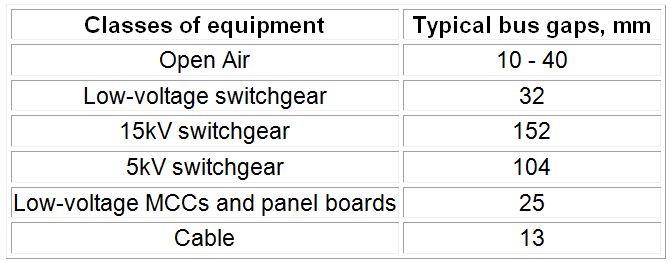
\includegraphics[width=5in, keepaspectratio=true]{../Images/Gaps.png} \\
\end{center}

\noindent\textbf{Gap between Conductors } \\  
\noindent Equipment bus gap in mm. Gaps of 3 to 40 mm are used for low voltage testing to simulate gaps between conductors in low voltage equipment and cables. Gaps 13, 104 and 152 mm. are used in 5 and 15kV equipment testing.\\
   
\noindent\textbf{Grounding Type}    \\
\noindent Two grounding classes are applied in the IEEE 1584 procedure, as follows:
\begin{enumerate}
	\item Ungrounded, this included ungrounded, high-resistance grounding and low-resistance grounding.
	\item Solidly grounded. 
\end{enumerate}

\noindent\textbf{Working Distance }  \\ 
\noindent Typical working distance is the sum of the distance between the workers standing in front of the equipment, and from the front of the equipment to the potential arc source inside the equipment. \\

\noindent Arc-flash protection is always based on the incident energy level on the person's face and body at the working distance, not the incident energy on the hands or arms. The degree of injury in a burn depends on the percentage of a person's skin that is burned. The head and body are a large percentage of total skin surface area and injury to these areas is much more life threatening than burns on the extremities. \\

\noindent Typical working distances are shown in table below:
\begin{center}
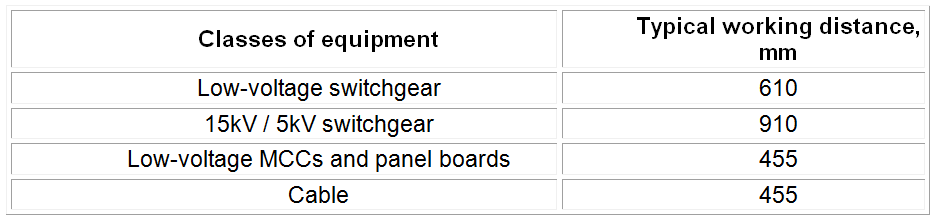
\includegraphics[width=5in, keepaspectratio=true]{../Images/WorkingDistance.png} \\
\end{center}

\noindent\textbf{Arc Duration / Total Clearing Time   } \\
\noindent Protective device characteristics, which can be found in the manufacturers, supplied data. For fuses, the manufacturer's time-current curves may include both melting and clearing time. In such a case, the clearing time is used. If they show only the average melt time, 15\% is added to that time, up to 0.03 seconds, and 10\% above 0.03 seconds to determine total clearing time. If the arcing fault current is above the total clearing time at the bottom of the curve (0.01 seconds), 0.01 seconds is used for the time. \\
For circuit breakers with integral trip units, the manufacturer's time-current curves include both tripping time and clearing time. \\

\noindent For relay operated circuit breakers, the relay curves show only the relay operating time in the time-delay region. For relays operating in their instantaneous region, 16 milliseconds are typically allowed on 60 Hz systems for operation. The circuit breaker opening time must be added. Opening times for particular circuit breakers can be verified by consulting the manufacturer's literature. \\
 
  
\noindent\textbf{Available 3 Phase Bolted Fault Current}  \\ 
Available 3 phase bolted fault current for each specific location as determined by the Short Circuit Analysis. \\
 
\noindent\emph{NOTE: Effect of arc current variation on determination of clearing time:    
For protective devices operating in the steep portion of their time-current curves, a small change in current causes a big change in operating time. Incident energy is linear with time, so arc current variation may have a big effect on incident energy. The solution is to make two arc current and energy calculations; one using the calculated expected arc current and one using a reduced arc current that is 15\% lower.}\\ 

%Observations
\section{Observations}
\label{af:observations}

\subsection{Arc Flash Hazard Study Detailed Results}
\label{af:observations:at}

Please refer to Arc Flash Report Table for detailed Arc Flash Analysis Results.

\pagebreak

\subsection{Power Distribution System Single Line Diagrams}
\label{af:observations:sld}

The following pages depict a detailed Equipment Single Line Diagram (SLD) and Arc Flash Hazard SLD.

\begin{thebibliography}{1}

\bibitem{IEEE} Institute of Electrical and Electronics Engineers {\em Std 1584: IEEE Guide for Performing Arc Flash Hazard Calculations}  2002.
\bibitem{CSA} CSA {\em Z462-15: Workplace Electrical Safety}  2015.
\bibitem{NFPA} NFPA {\em NFPA 70E: Standard for Electrical Safety in the Workplace and Handbook}  2015.

\end{thebibliography}

\end{document}

